% ============================================================================
% EdgeVLM Lab -- mid-project report: Lucius's sections (3, 5, 6)
% Paste each section into 1-main-midproject.tex in place of the template's
% Section 3 / 5 / 6. Upload architecture.png, dataflow.png and tradeoff.png to
% the same Overleaf folder. Table I is already filled in from results.json.
% All numbers are filled in. SmolVLM's answer time stays "pending" until the
% model is connected to /api/ask.
% Lines marked  % ANH:  are for Anh.
% Length: about 2 pages in two-column format, leaving room for Sections 1, 2, 4.
% ============================================================================

\section{Technical System Architecture \& Data Flow}
\label{sec:arch}

Figure~\ref{fig:arch} shows how data moves through EdgeVLM Lab. A \emph{live}
path runs on every interaction and follows the four required stages:
UI inputs $\rightarrow$ execution hooks/API $\rightarrow$ tensor processing
$\rightarrow$ visual rendering. An \emph{offline} path (RTL verification, logic
synthesis, model profiling) runs once, and its results are stored as JSON.
Keeping the slow work offline is what lets the live path respond quickly
(Section~\ref{sec:latency}).

\begin{figure*}[t]
  \centering
  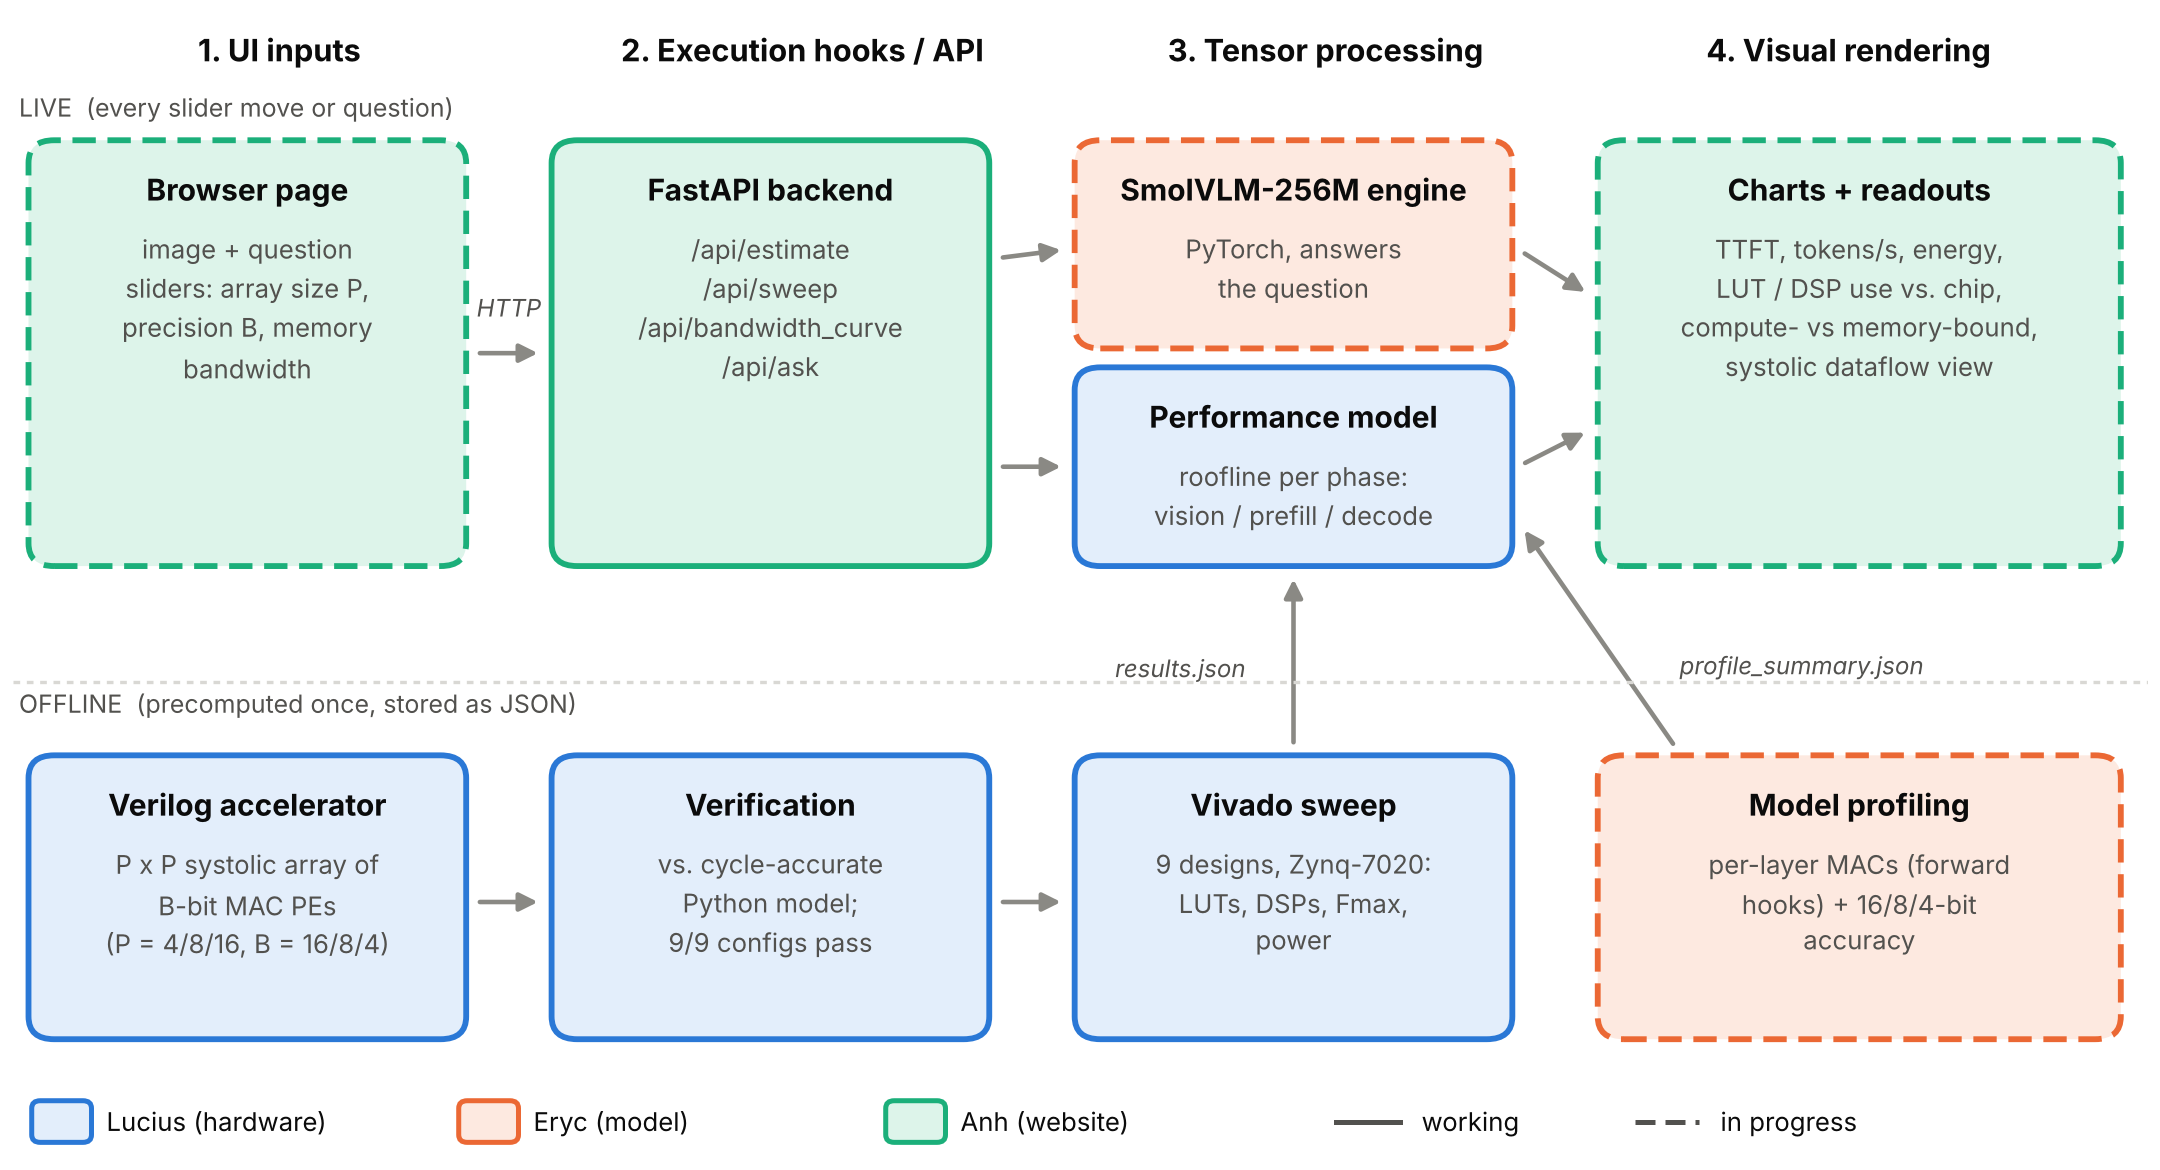
\includegraphics[width=0.92\textwidth]{architecture.png}
  \caption{System architecture. Top: live path, run on every slider move or
  question. Bottom: offline path, whose JSON outputs the backend reloads
  automatically when they change. Solid borders mark working components;
  dashed borders mark components in progress.}
  \label{fig:arch}
\end{figure*}

\textbf{Frontend and backend.} A FastAPI backend serves the page. Moving a
slider sends the array size $P$, precision $B$ and memory bandwidth as JSON to
\texttt{/api/estimate}. \texttt{/api/sweep} returns all nine designs, and
\texttt{/api/bandwidth\_curve} returns tokens/s as bandwidth varies. The
backend calls the performance model directly, without changing its output. It
caches the hardware and workload JSON files until they change on disk, and
it marks every response with which numbers are still placeholders.
% ANH: one sentence on the frontend framework and how it renders the charts.

\textbf{Accelerator.} Almost all of a transformer's computation is matrix
multiplication, so our hardware is a $P \times P$ output-stationary systolic
array~\cite{kung1982systolic} in parameterized Verilog. Each processing
element (PE) has a signed $B$-bit multiplier and an accumulator. Every cycle it
adds $a \cdot b$ into its accumulator and passes $a$ right and $b$ down. Row $i$
of $A$ is delayed $i$ cycles and column $j$ of $B$ is delayed $j$ cycles, so
$A_{ik}$ and $B_{kj}$ meet in PE$(i,j)$ at cycle $k+i+j$
(Fig.~\ref{fig:dataflow}). Each operand is fetched once and reused $P$ times,
the same idea used in the TPU~\cite{jouppi2017tpu}. A $P\times P$ output tile
with inner dimension $K$ takes
\begin{equation}
  T_{\text{tile}} = K + 2P - 2 \ \text{cycles}.
  \label{eq:tile}
\end{equation}
One source file produces all nine designs ($P \in \{4,8,16\}$,
$B \in \{16,8,4\}$). The accumulator is $2B+12$ bits, which cannot overflow
for any $K \le 8191$. SmolVLM's largest inner dimension is 3072.

\begin{figure}[t]
  \centering
  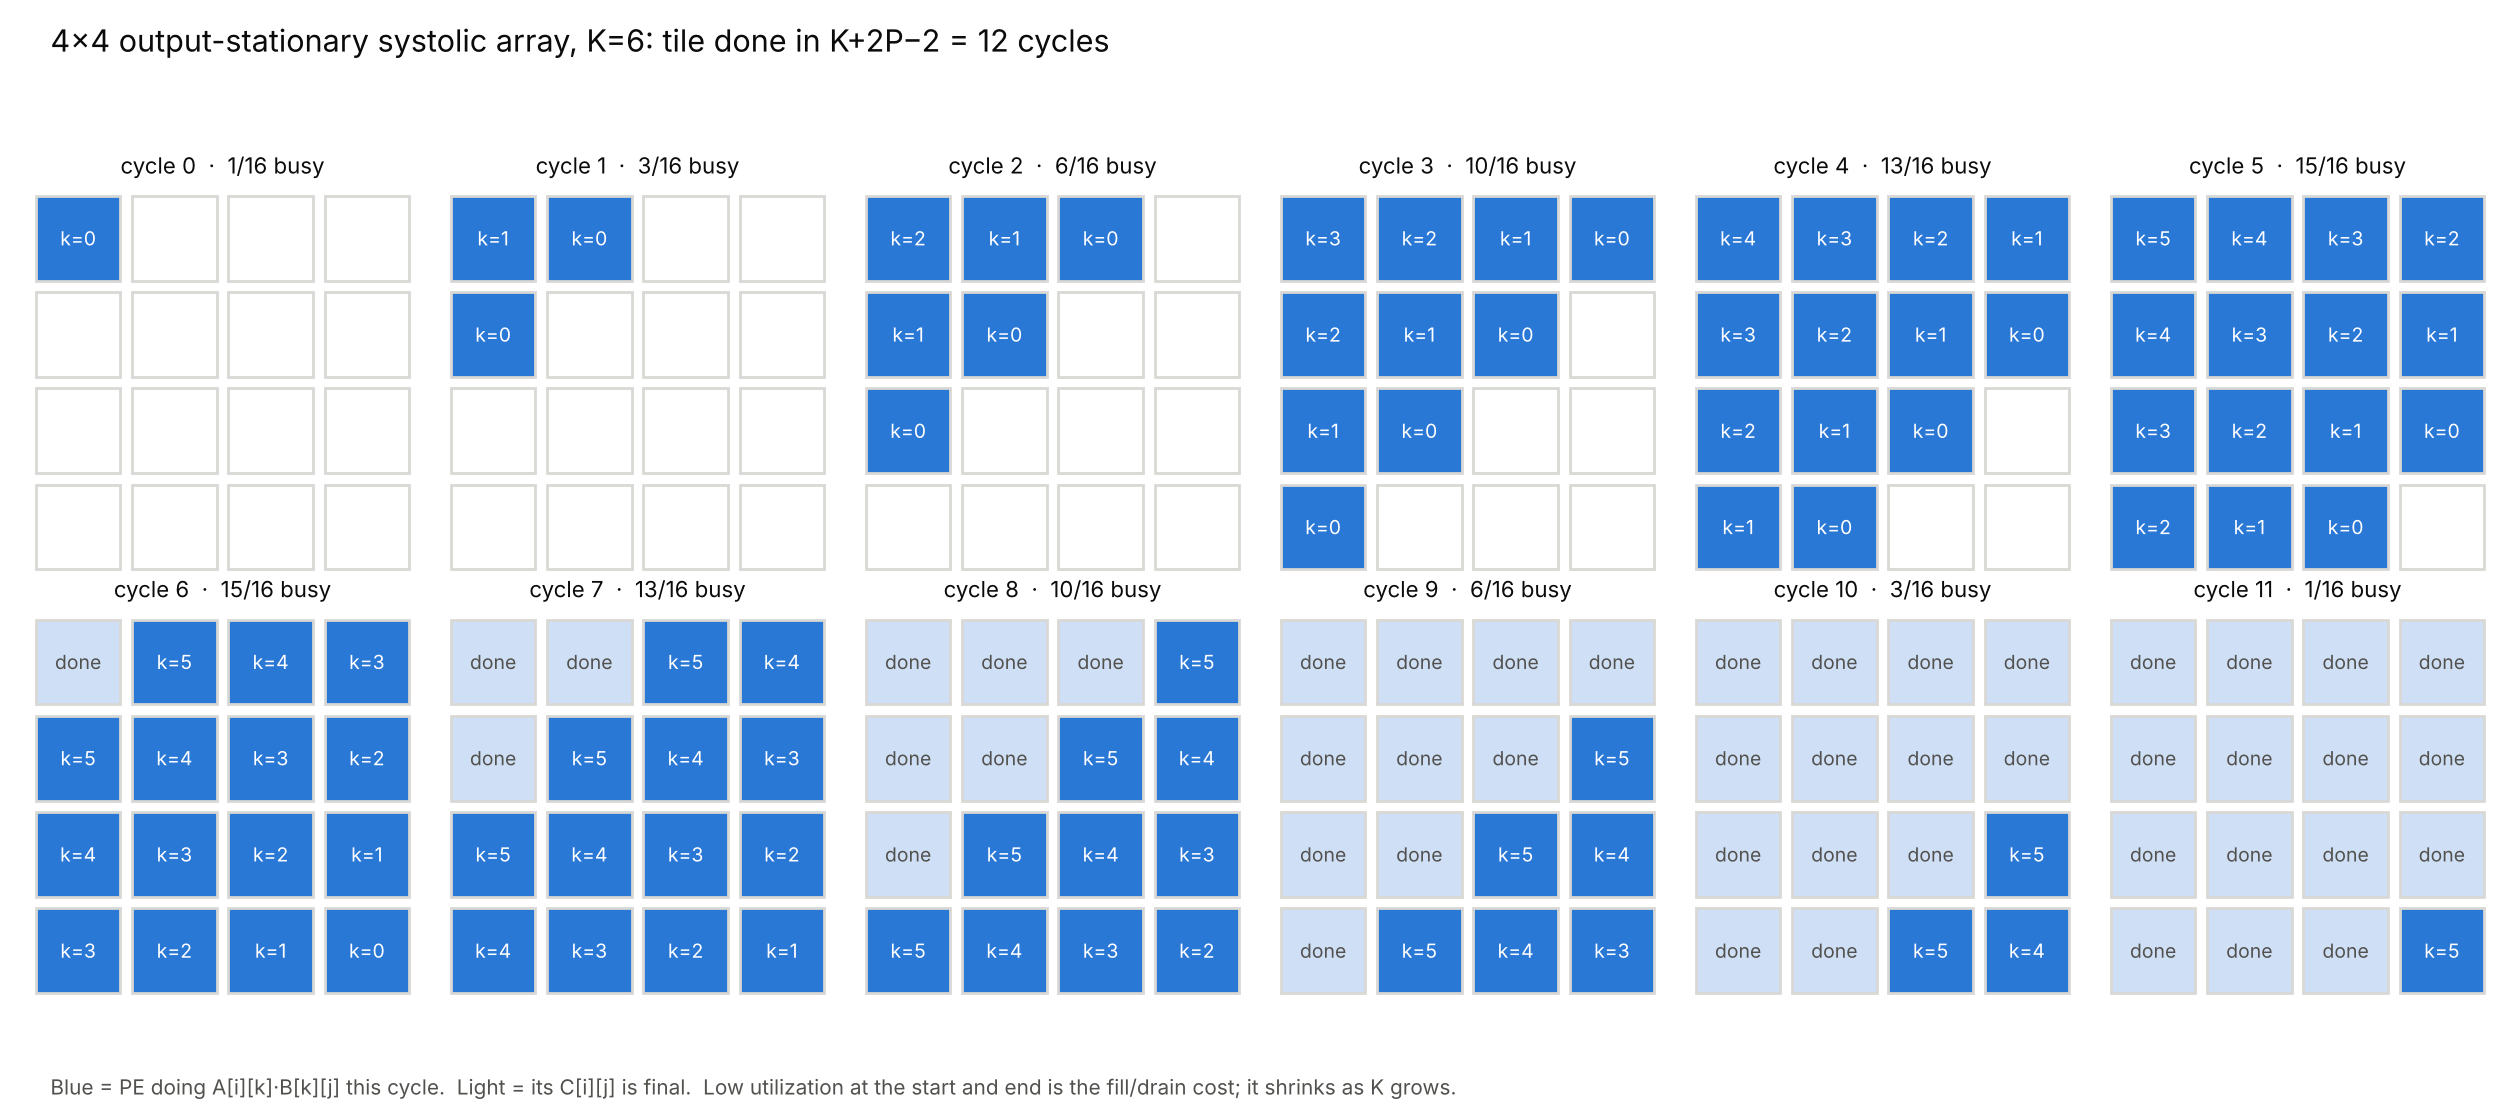
\includegraphics[width=\columnwidth]{dataflow.png}
  \caption{Cycle-by-cycle dataflow of a $4\times4$ array ($K=6$) from our
  cycle-accurate model. Blue: PE multiplying $A_{ik}B_{kj}$ in that cycle;
  light: result final. The tile finishes in $K+2P-2=12$ cycles. This is the
  lowest level of the tool's multi-level view (G2).}
  \label{fig:dataflow}
\end{figure}

\textbf{Verification.} A cycle-accurate Python model mirrors the RTL register
by register and matches NumPy on 18 $(P,B)$ configurations. A self-checking
testbench streams random signed matrices, with idle cycles in the middle, and
compares every output against a behavioral multiply. All nine designs pass,
as do runs with $K$ up to 3072. Its first trial uses the worst-case operand
$-2^{B-1}$ everywhere. This test caught a real bug: our original $2B+8$-bit
accumulator got all 16 outputs wrong at $K=600$, which is smaller than several
real layers.

\textbf{Synthesis.} Each design is synthesized out of context for the
Zynq-7020 (\texttt{xc7z020clg484-1}: 53{,}200 LUTs, 220 DSPs) at a 100~MHz
constraint. A script collects resources, worst negative slack (WNS) and
estimated power into \texttt{results.json}, with
$f_{\max} = 1/(10\,\text{ns} - \text{WNS})$. These are post-synthesis
estimates. Three patterns stand out (Table~\ref{tab:designs}).
(i)~At 16~bits, Vivado maps each whole PE (multiplier, accumulator and operand
registers) into one DSP48E1 slice, so the $4\times4$ and $8\times8$ designs
use almost no LUTs and reach an estimated 296~MHz.
(ii)~At 8 and 4~bits, Vivado builds the multipliers from LUTs instead
(0 DSPs): about 90 and 38 LUTs per PE, at 130 and 162~MHz.
(iii)~For a given precision, $f_{\max}$ does not change with $P$. A systolic
array only has short wires between neighbors, so its critical path stays
inside one PE. The exception is $16\times16$ at 16~bits, which needs 256
multipliers: Vivado used all 220 DSPs, built the other 36 from LUTs, and missed
the 100~MHz target (94.9~MHz). All nine designs fit the device; the largest
uses 43\% of its LUTs. Power is a vectorless estimate (0.12--0.52~W) and
mostly static.

% --- Table I (generated by perf/report_table.py from results.json) ---------
\begin{table}[t]
\centering
\small
\setlength{\tabcolsep}{3.5pt}
\caption{The nine designs on the Zynq-7020 (Vivado, post-synthesis) and their predicted TTFT and decode speed at each design's $f_{\max}$, 1~GB/s (placeholder workload).}
\label{tab:designs}
\begin{tabular}{l c r r r r r r}
\hline
Array & Bits & LUTs & DSPs & $f_{\max}$ & Power & TTFT & Tok/s \\
      &      &      &      & (MHz)      & (W)   & (s)  &       \\
\hline
$4\times4$ & 16 & 25 & 16 & 295.9 & 0.121 & 28.27 & 3.7 \\
$8\times8$ & 16 & 123 & 64 & 295.9 & 0.179 & 7.27 & 3.7 \\
$16\times16$ & 16 & 12,158 & 220 & 94.9 & 0.517 & 5.73 & 3.7 \\
$4\times4$ & 8 & 1,433 & 0 & 130.2 & 0.137 & 63.76 & 7.4 \\
$8\times8$ & 8 & 5,754 & 0 & 130.2 & 0.213 & 16.04 & 7.4 \\
$16\times16$ & 8 & 22,842 & 0 & 130.2 & 0.522 & 4.11 & 7.4 \\
$4\times4$ & 4 & 610 & 0 & 162.2 & 0.117 & 51.14 & 14.8 \\
$8\times8$ & 4 & 2,427 & 0 & 162.2 & 0.149 & 12.84 & 14.8 \\
$16\times16$ & 4 & 9,836 & 0 & 161.5 & 0.274 & 3.27 & 14.8 \\
\hline
\end{tabular}
\end{table}
% -----------------------------------------------------------------------------

\textbf{Performance model.} We combine the workload with each design using a
per-phase roofline~\cite{williams2009roofline}:
\begin{equation}
  t = \max\!\left( \frac{\text{MACs}}{P^2 f\,u},\;
                   \frac{\text{bytes}}{\text{BW}} \right),
  \label{eq:roofline}
\end{equation}
where $f$ is the clock, $u$ the PE utilization and BW the memory bandwidth.
Weights take $B/8$ bytes each. SmolVLM~\cite{marafioti2025smolvlm} answers in
three phases: the vision encoder, prefill over the image and prompt tokens,
and token-by-token decode, which re-reads every language-model weight for
each token. TTFT $= t_{\text{vision}} + t_{\text{prefill}} + t_{\text{decode}}$
and tokens/s $= 1/t_{\text{decode}}$.

Figure~\ref{fig:tradeoff} shows the tool's central lesson. Decode does about
one MAC per weight byte, so it is memory-bound: array size leaves tokens/s
unchanged, and only fewer bits raise it (3.7, 7.4 and 14.8 tokens/s at 16, 8
and 4 bits). Vision and prefill are compute-bound, so TTFT falls with array
size: at 4~bits, from 51~s at $4\times4$ to 3.3~s at $16\times16$, close to
the $P^2=16\times$ expected. The synthesis results add a twist that users can
discover with the sliders: fewer bits do not always give a faster first
token. 16-bit PEs run in DSP slices at 296~MHz while 8-bit PEs run in LUTs at
130~MHz, so at $4\times4$ and $8\times8$ the 16-bit design has the
\emph{shortest} TTFT (28~s vs.\ 64~s at $4\times4$). Packing two 8-bit
multiplies into each DSP would remove this penalty. Overall, $16\times16$ at
4~bits is best on every axis: 3.3~s TTFT, 14.8 tokens/s and 1.5~J of
accelerator energy per 32-token answer. The workload is still a placeholder
(Section~\ref{sec:roadmap}), so the trends hold but the absolute numbers
will change.

\begin{figure}[t]
  \centering
  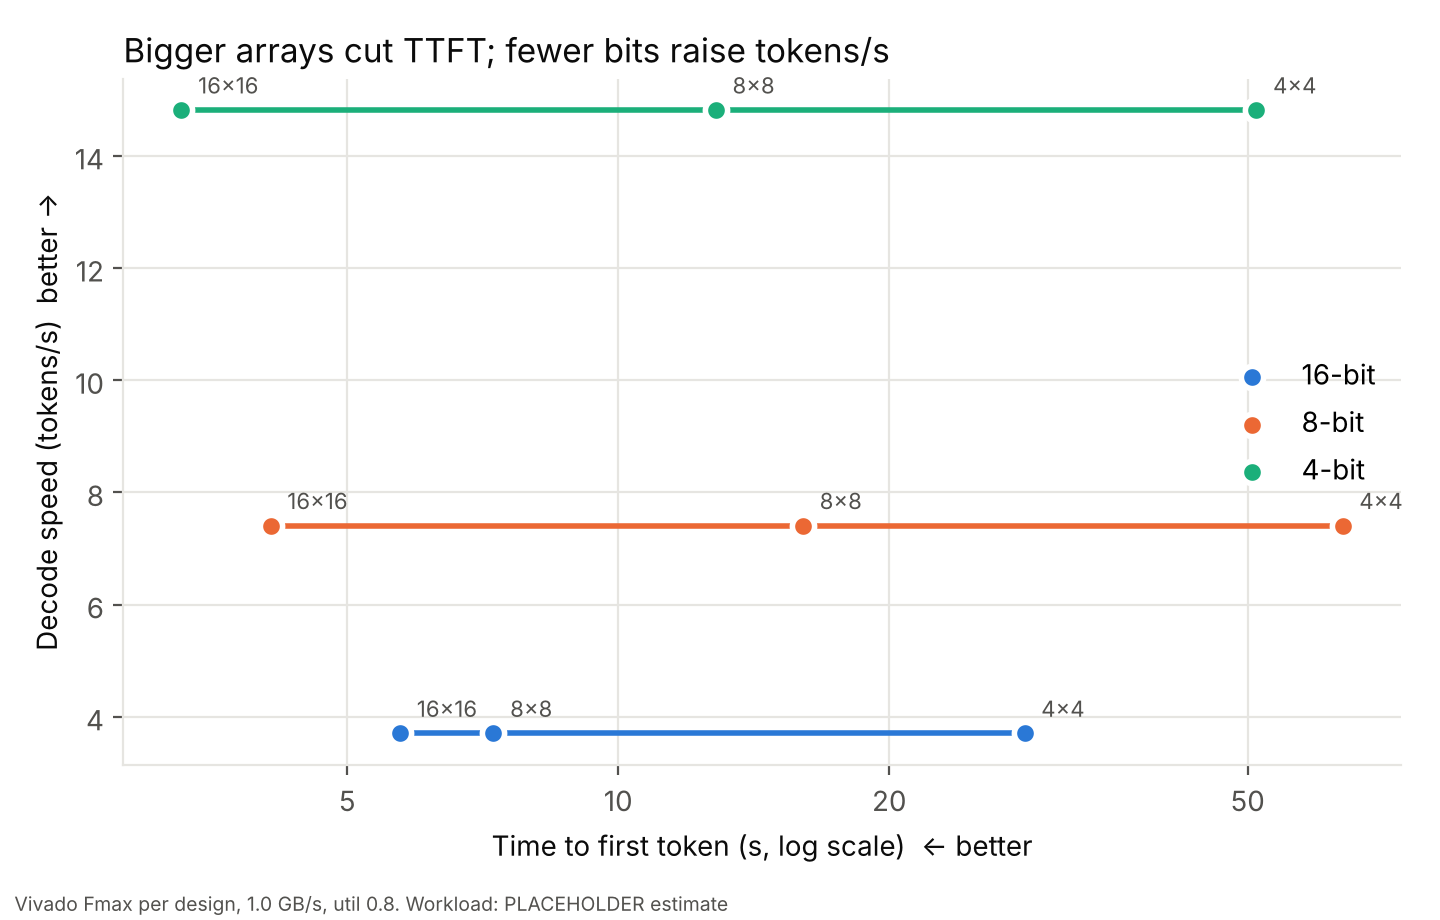
\includegraphics[width=\columnwidth]{tradeoff.png}
  \caption{Predicted TTFT vs.\ decode speed for the nine designs, each at its
  Vivado $f_{\max}$ (placeholder workload, 1~GB/s). Fewer bits move designs
  up; larger arrays move them left. The 16-bit line flattens at
  $16\times16$ because 36 of its multipliers spill out of DSPs into LUTs.}
  \label{fig:tradeoff}
\end{figure}

% ============================================================================
\section{Compute, Latency \& Optimization Analysis}
\label{sec:latency}

This section is about the tool's own response time, meaning how quickly a
slider move updates the display. It is separate from the accelerator latency
the tool predicts. Table~\ref{tab:latency} gives preliminary measurements
(\texttt{perf/measure\_latency.py} on a Windows PC: 1{,}000 calls to the
model, 50 HTTP requests per endpoint). The performance model is closed-form,
so all nine designs take 8~$\mu$s. A full slider update through the backend
takes about 1--3~ms (median), far below the $\sim$100~ms at which a
response stops feeling instant. The cost is the HTTP round trip, not the
computation.

\begin{table}[t]
\centering
\small
\caption{Preliminary response times: median (95th percentile).}
\label{tab:latency}
\begin{tabular}{l r}
\hline
Operation & Time \\
\hline
Performance model, all 9 designs & 0.008 ms \\
\texttt{/api/estimate} (one slider move) & 1.1 (23.9) ms \\
\texttt{/api/sweep} (all 9 designs) & 3.2 (22.7) ms \\
\texttt{/api/bandwidth\_curve} (120 points) & 2.3 (26.3) ms \\
SmolVLM answer, CPU (one question) & pending \\
Vivado synthesis, all 9 designs (offline) & 7.9 min \\
\hline
\end{tabular}
\end{table}

\textbf{Strategies.} (1)~\emph{Precompute the slow paths:} synthesis takes
about 8 minutes for all nine designs (28--126~s each), so it runs once and is
served from JSON,
and model profiling works the same way. (2)~\emph{Closed-form model:}
Eq.~(\ref{eq:roofline}) needs no simulation, so all designs, or a whole
bandwidth curve, update in one request. (3)~\emph{Caching:} the backend
reloads JSON only when files change. Next we will cache each image's vision
embedding so follow-up questions skip the most expensive phase.
(4)~\emph{Quantized, in-browser inference (planned):} an 8-bit
SmolVLM~\cite{jacob2018quantization} running in the browser (ONNX/WebGPU)
removes the server round trip. (5)~\emph{Use 127.0.0.1, not localhost:} our first
measurement showed 2.07~s per request. On Windows, \texttt{localhost}
resolves to IPv6 first while the server listens on IPv4, so every request
waited for a failed connection; addressing the server by 127.0.0.1 brought
it to 1.1~ms. (6)~\emph{Fast simulation:} replacing the array's
flat internal buses with one wire per link made $16\times16$ simulation more
than $60\times$ faster, so per-cycle traces for the dataflow animation can be
precomputed.

% ============================================================================
\section{Technical Roadblocks \& 5-Week Execution Roadmap}
\label{sec:roadmap}

\textbf{Roadblocks.}
(1)~\emph{Accumulator overflow:} found by the worst-case test and fixed by
adding 4 bits (Section~\ref{sec:arch}).
(2)~\emph{DSP limit:} a $16\times16$ array needs 256 multipliers but the chip
has 220 DSPs, so at 16~bits Vivado built 36 of them from LUTs and the design
missed 100~MHz. Larger arrays will need DSP packing, tiling or a bigger device.
(2b)~\emph{Low-precision mapping:} 8- and 4-bit multipliers land in LUTs at
a lower clock, which erases part of their benefit for prefill.
(3)~\emph{Placeholder workload:} SmolVLM splits large images into sub-images,
so the real number of image tokens, and therefore TTFT, may be several times
the placeholder until profiling is done.
(4)~\emph{Simulator scaling:} simulation time grew roughly as $P^4$ until we
restructured the wiring. (4b)~\emph{2-second requests:} a Windows
\texttt{localhost}/IPv6 issue added 2~s to every API call until we addressed
the server by 127.0.0.1 (Section~\ref{sec:latency}).
(5)~\emph{Integration:} the model is not yet connected to \texttt{/api/ask}.

\textbf{Week-by-week plan} (L = Lucius, E = Eryc, A = Anh).
\begin{itemize}
  \setlength{\itemsep}{1pt}
  \item \textbf{Nov 2--8.} L: check the performance model against a
        cycle-accurate run of a full $576\times576$ layer. E: real profile
        and 16/8/4-bit accuracy; connect SmolVLM to \texttt{/api/ask}.
        A: finish the sliders and placeholder labels.
  \item \textbf{Nov 9--15.} L: add attention matmuls and activation traffic;
        pack two 8-bit multiplies per DSP; place-and-route two designs to
        check $f_{\max}$. E: per-layer
        quantization sensitivity. A: roofline chart, animated dataflow (G2).
  \item \textbf{Nov 16--22.} L: tile scheduler for full layers; Verilog
        download (stretch). E: cache image embeddings; in-browser inference.
        A: model layer map (G1).
  \item \textbf{Nov 23--29.} All: user study with 5--6 classmates (three
        tasks, e.g.\ ``find the cheapest design with TTFT under 10~s'', plus
        a usability questionnaire and before/after concept questions).
  \item \textbf{Nov 30--Dec 6.} All: fix issues from the study; final sweep
        and accuracy numbers; draft final report.
  \item \textbf{Dec 7--11.} All: final report, video, presentation.
\end{itemize}
